
\documentclass[8pt]{article}

\usepackage[utf8]{inputenc}

\usepackage{amsmath, bm}
\usepackage{graphicx}
\usepackage{amssymb}
\usepackage{float}
\usepackage{caption}
\usepackage{subcaption}
% set font size to 11pt

% set margin
\usepackage[margin=0.5in]{geometry}

\setlength{\parskip}{\baselineskip}%
\setlength{\parindent}{0pt}%
\setlength{\voffset}{-0.75in}
\setlength{\headsep}{5pt}

\begin{document}

% insert pdf cover page here

\title{Lab report: 3F1 Flight Control}
\author{lwp26}
\date{October 2023}
\maketitle

\begin{abstract}
    \centering
    This report investigates the flight control systems of 
\end{abstract}

\section{Introduction}

Modern control systems

\section{Manual Aircraft Control}

\subsection{Simplified Aircraft Model}

A simplified model for aircraft dynamics is given by the following equation:

\[
 \ddot{y}(t) + M\dot{y}(t) = Nx(t)
\]

Where the coefficient $M$ represents the aerodynamic damping and coefficient $N$ represents aerodynamic effectiveness of elevators.
The transfer function of this system is given by:

\begin{equation}
    G(s) = \frac{N}{s(s + M)}
\end{equation}

\subsection{Manual Control}

The model for manual control by a pilot is taken as a pure time delay $D$ and a gain $k$ and so for an input response $x(t)$ the output is given as $kx(t-D)$.


1. Use your Bode diagram to make a sketch of the Nyquist diagram.


2. Are you using any integral action? Give a brief explanation. What implications does this have for the accuracy of our pilot model?
3. Explain the oscillation of the feedback loop. How does your observed period of oscillation compare to the theoretical prediction of the feedback loop?
4. Can you give a rough guideline to the control system designer to make PIO less likely?
5. Was your manual control able to reduce the error compared to no input? Compare all three cases (manual control, no control, manual control with small movements).
6. Sketch the Nyquist diagram of $G_2$</font> (hint: it is exactly circular).
7. Explain, using the Nyquist criterion, why the feedback system is stable with a proportional gain greater than 0.5
8. Finally, show how the Nyquist diagram is modified if a small time delay $D$ is introduced to the system.
9. Explain your reasoning for this bound on $Q$


\subsection{Aims}

\begin{itemize}
\item To determine the 
\end{itemize}

\section{Results}

\newpage

\begin{figure}
    \centering
    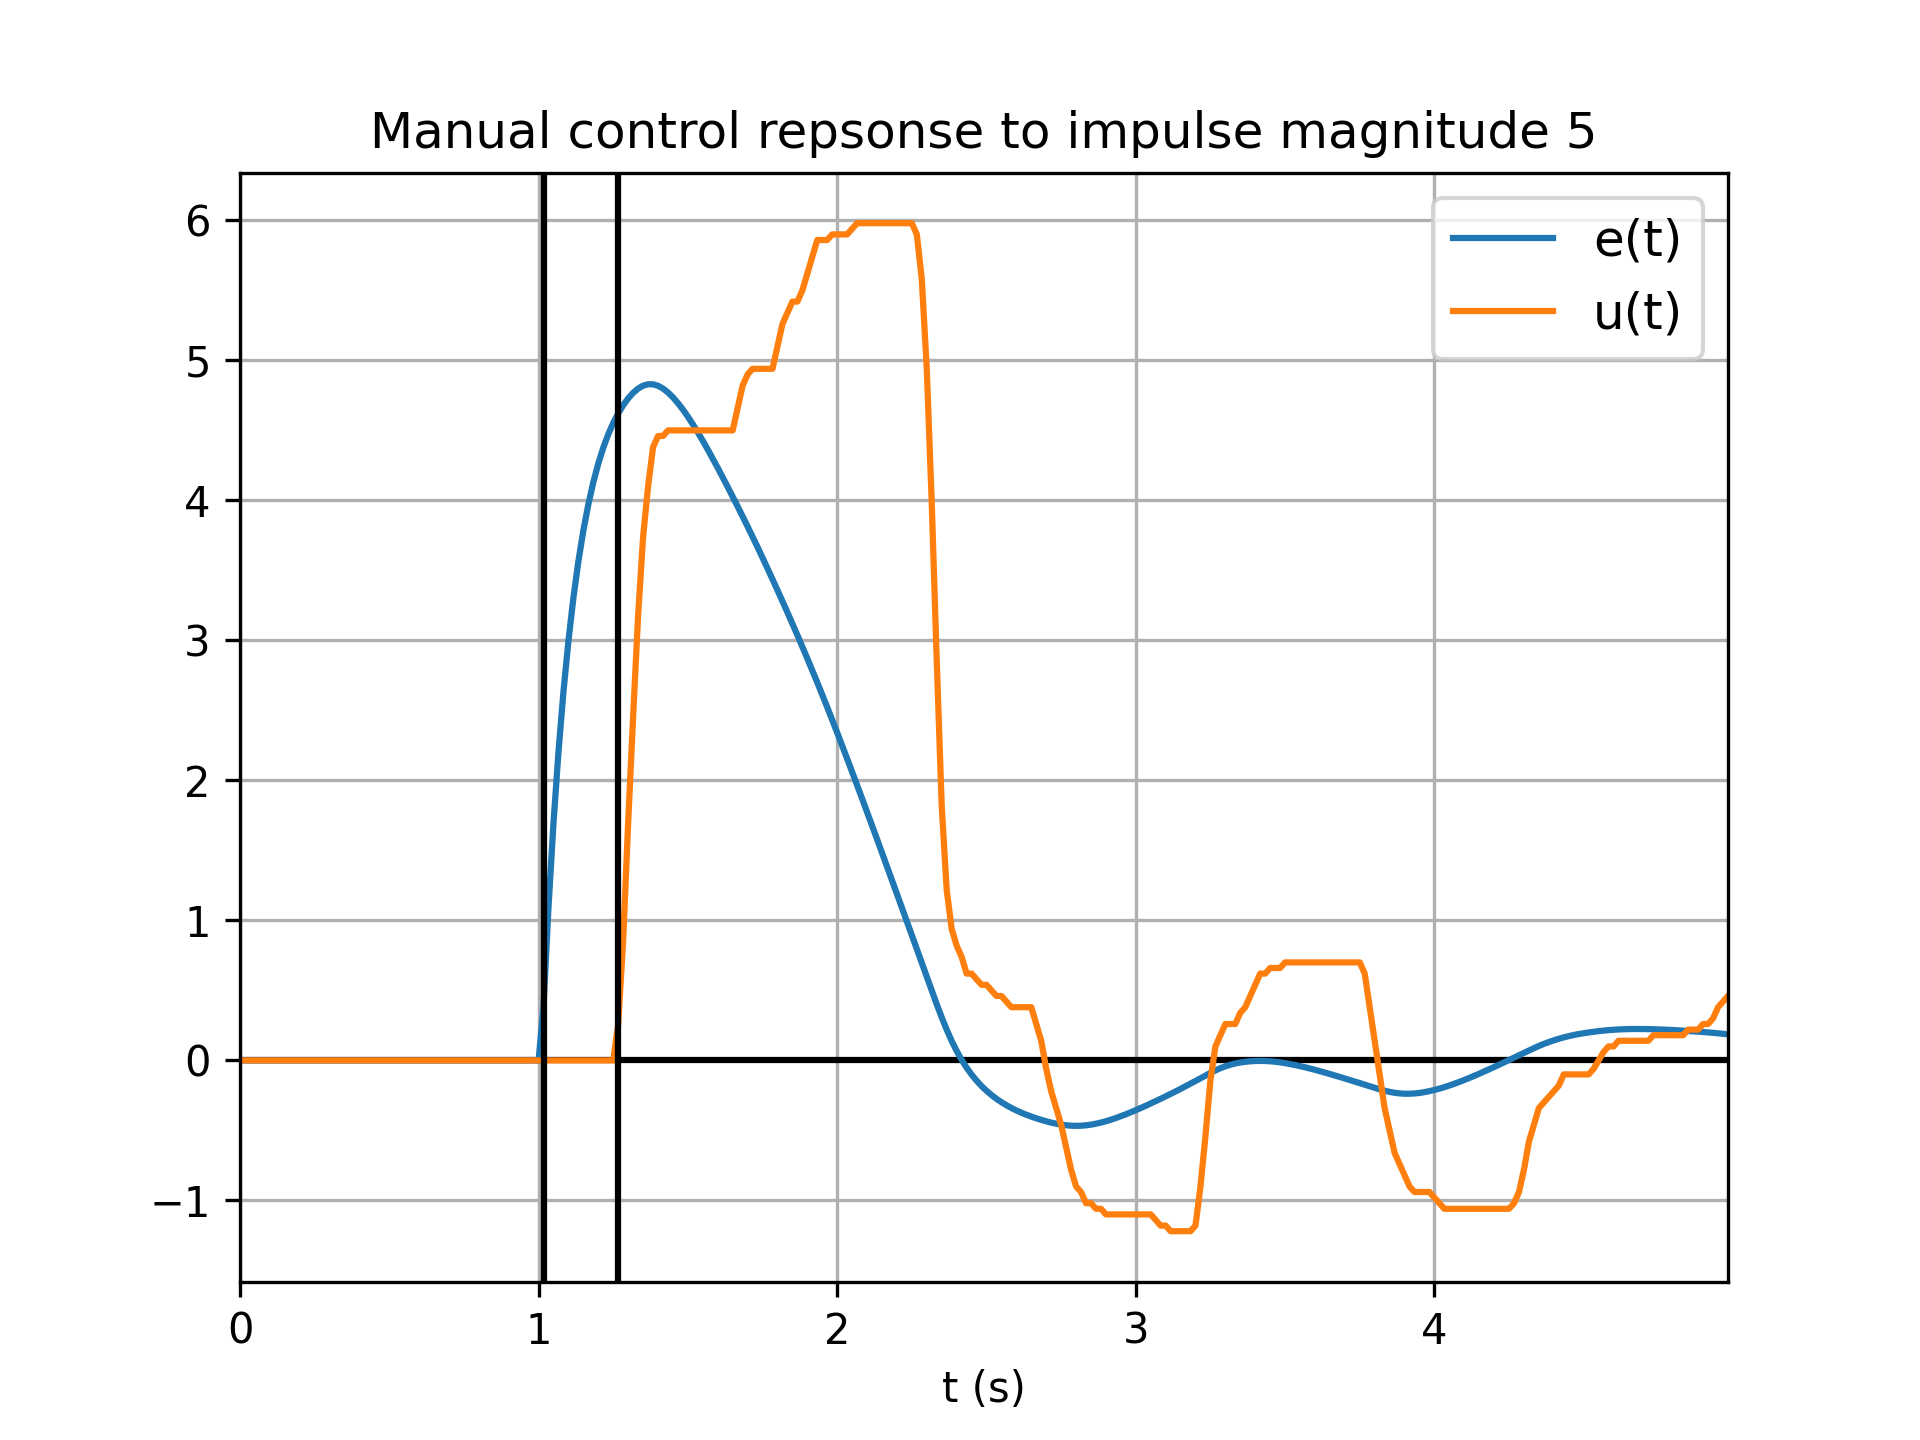
\includegraphics[width=0.8\textwidth]{figures/FIGURE_1.png}
    \caption{Figure 1}
    \label{fig:figure1}
\end{figure}

\begin{figure}
    \centering
    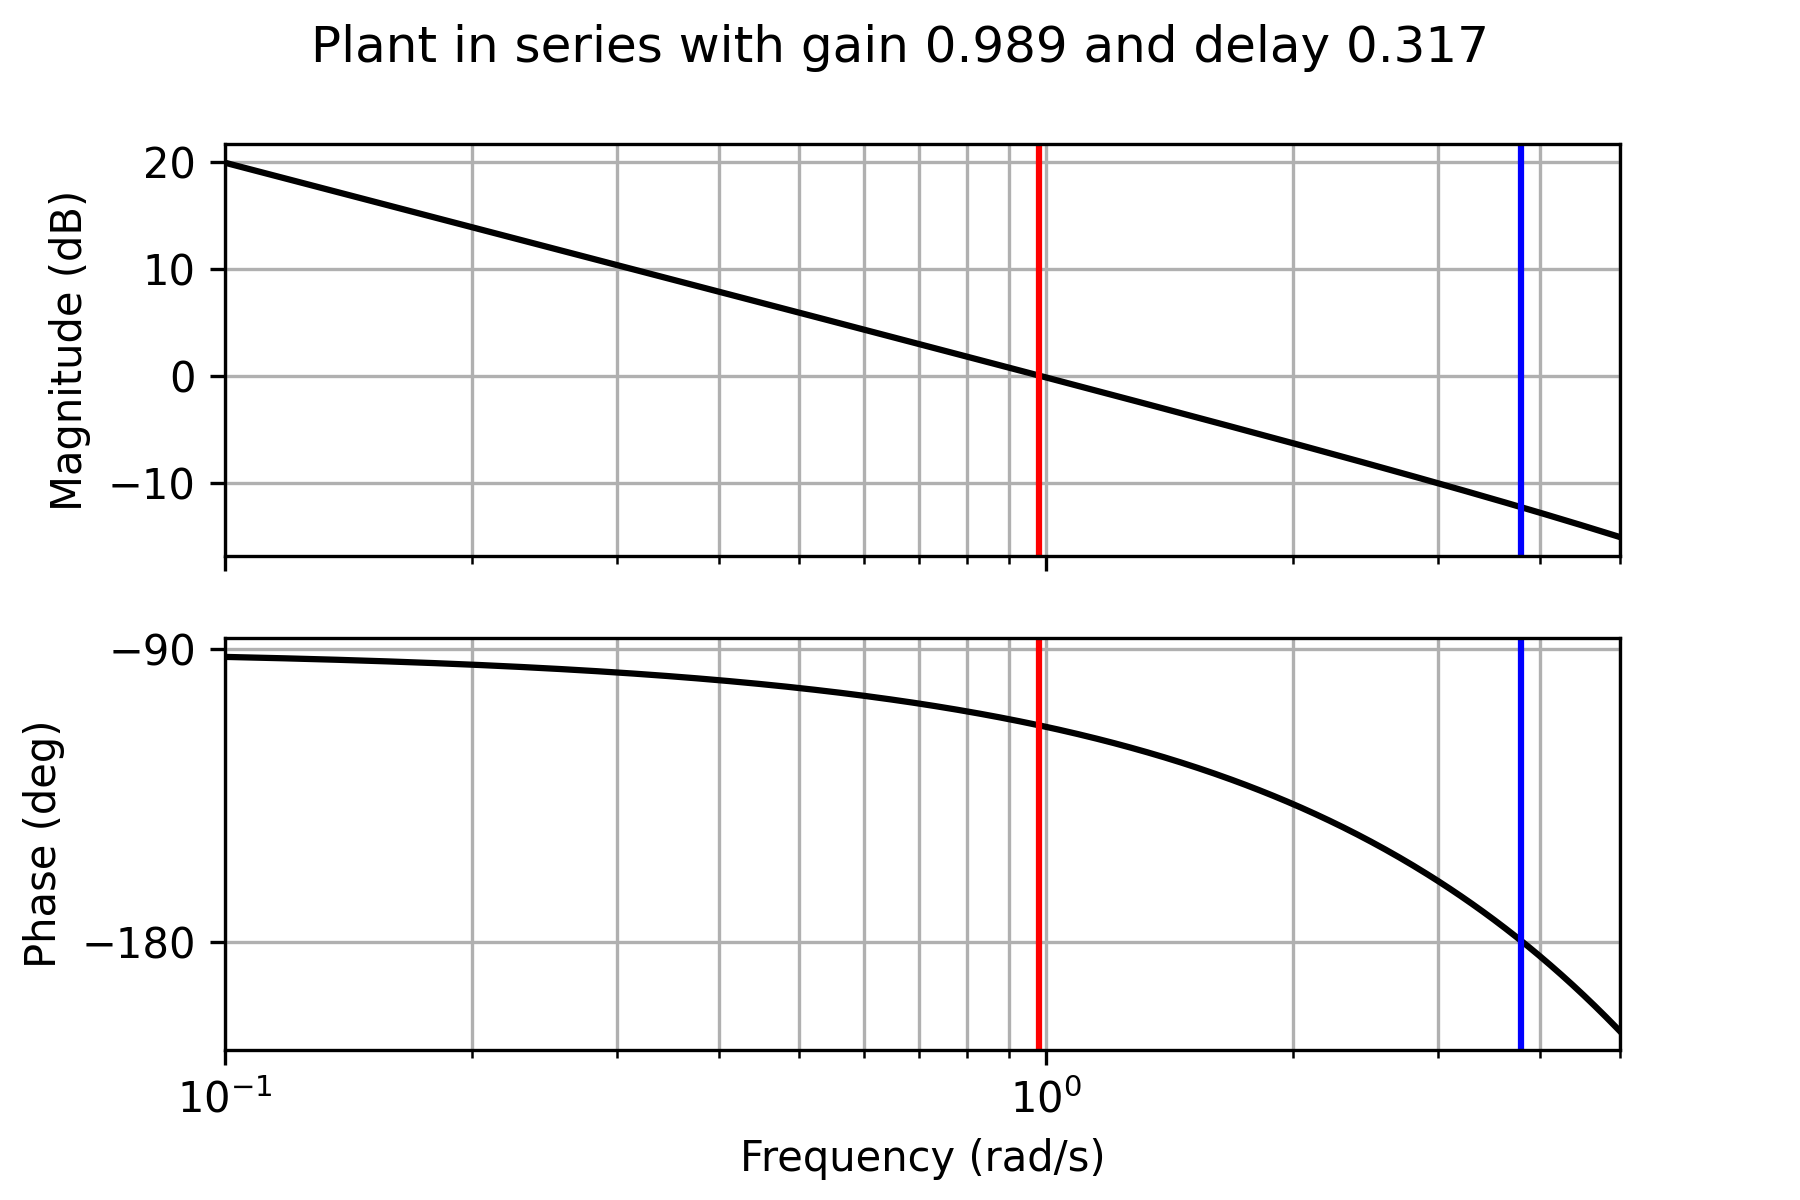
\includegraphics[width=0.8\textwidth]{figures/FIGURE_2.png}
    \caption{Figure 2}
    \label{fig:figure2}
\end{figure}

\newpage

\begin{figure}
    \centering
    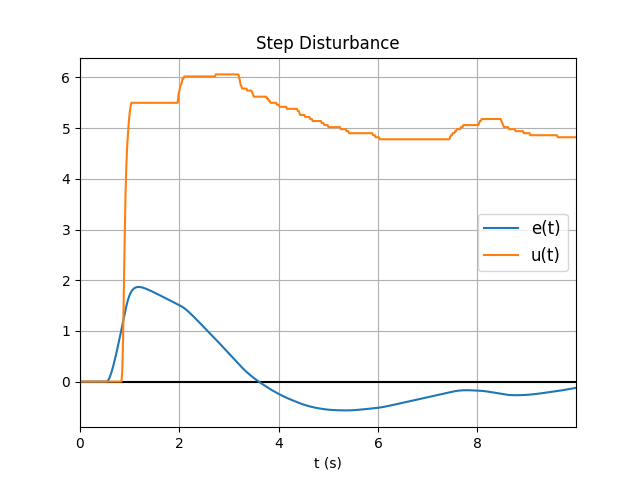
\includegraphics[width=0.8\textwidth]{figures/FIGURE_3.png}
    \caption{Figure 3}
    \label{fig:figure3}
\end{figure}

\newpage

\begin{figure}
    \centering
    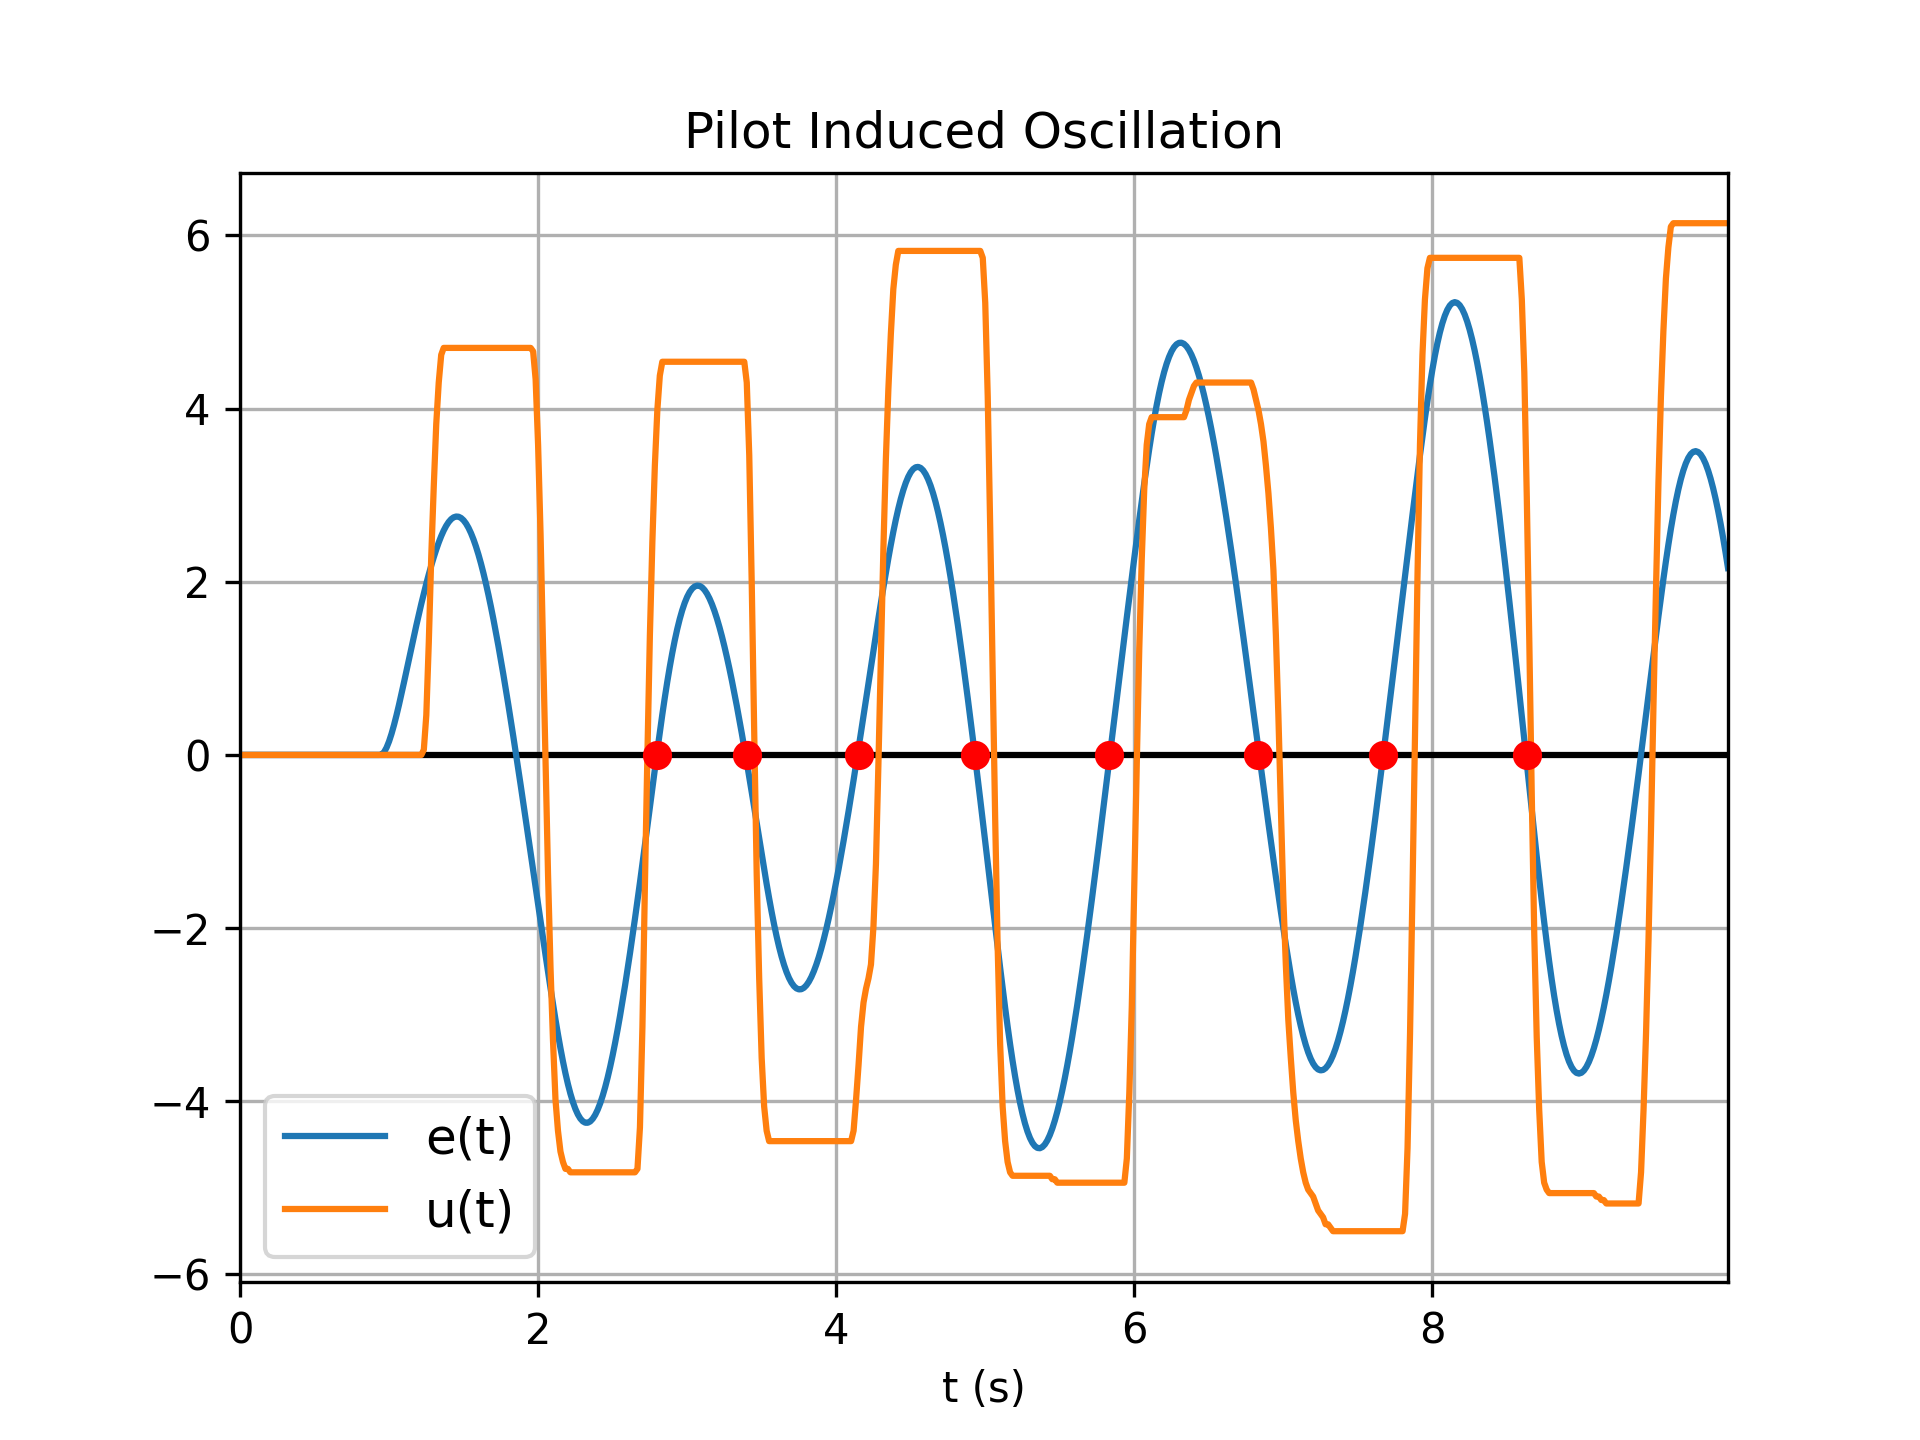
\includegraphics[width=0.8\textwidth]{figures/FIGURE_4.png}
    \caption{Figure 4}
    \label{fig:figure4}
\end{figure}

\begin{figure}
    \centering
    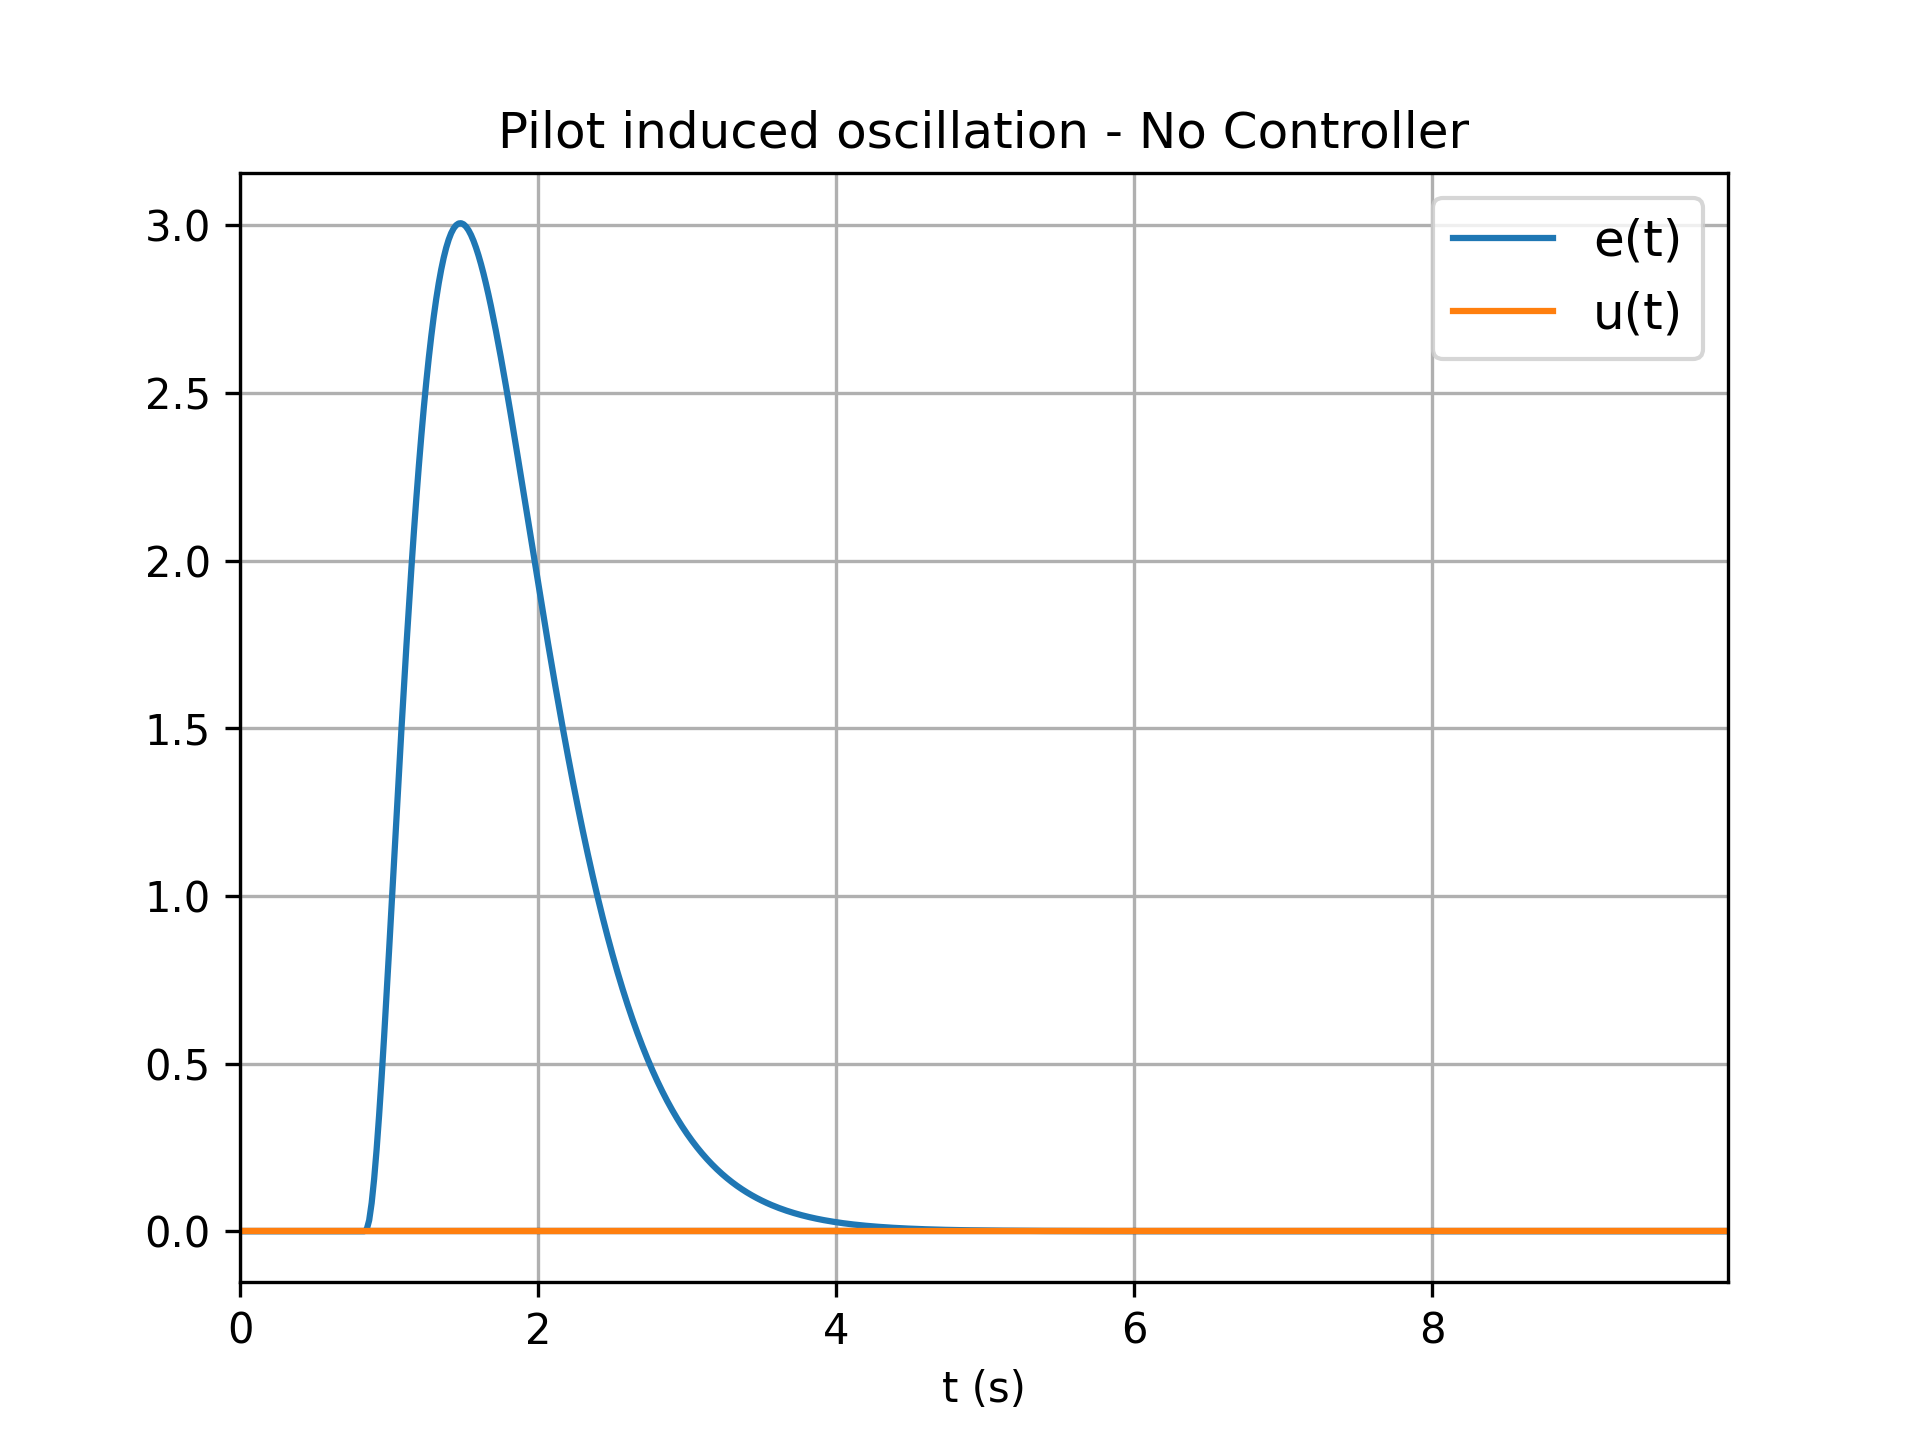
\includegraphics[width=0.8\textwidth]{figures/FIGURE_5.png}
    \caption{Figure 5}
    \label{fig:figure5}
\end{figure}

\newpage

\begin{figure}
    \centering
    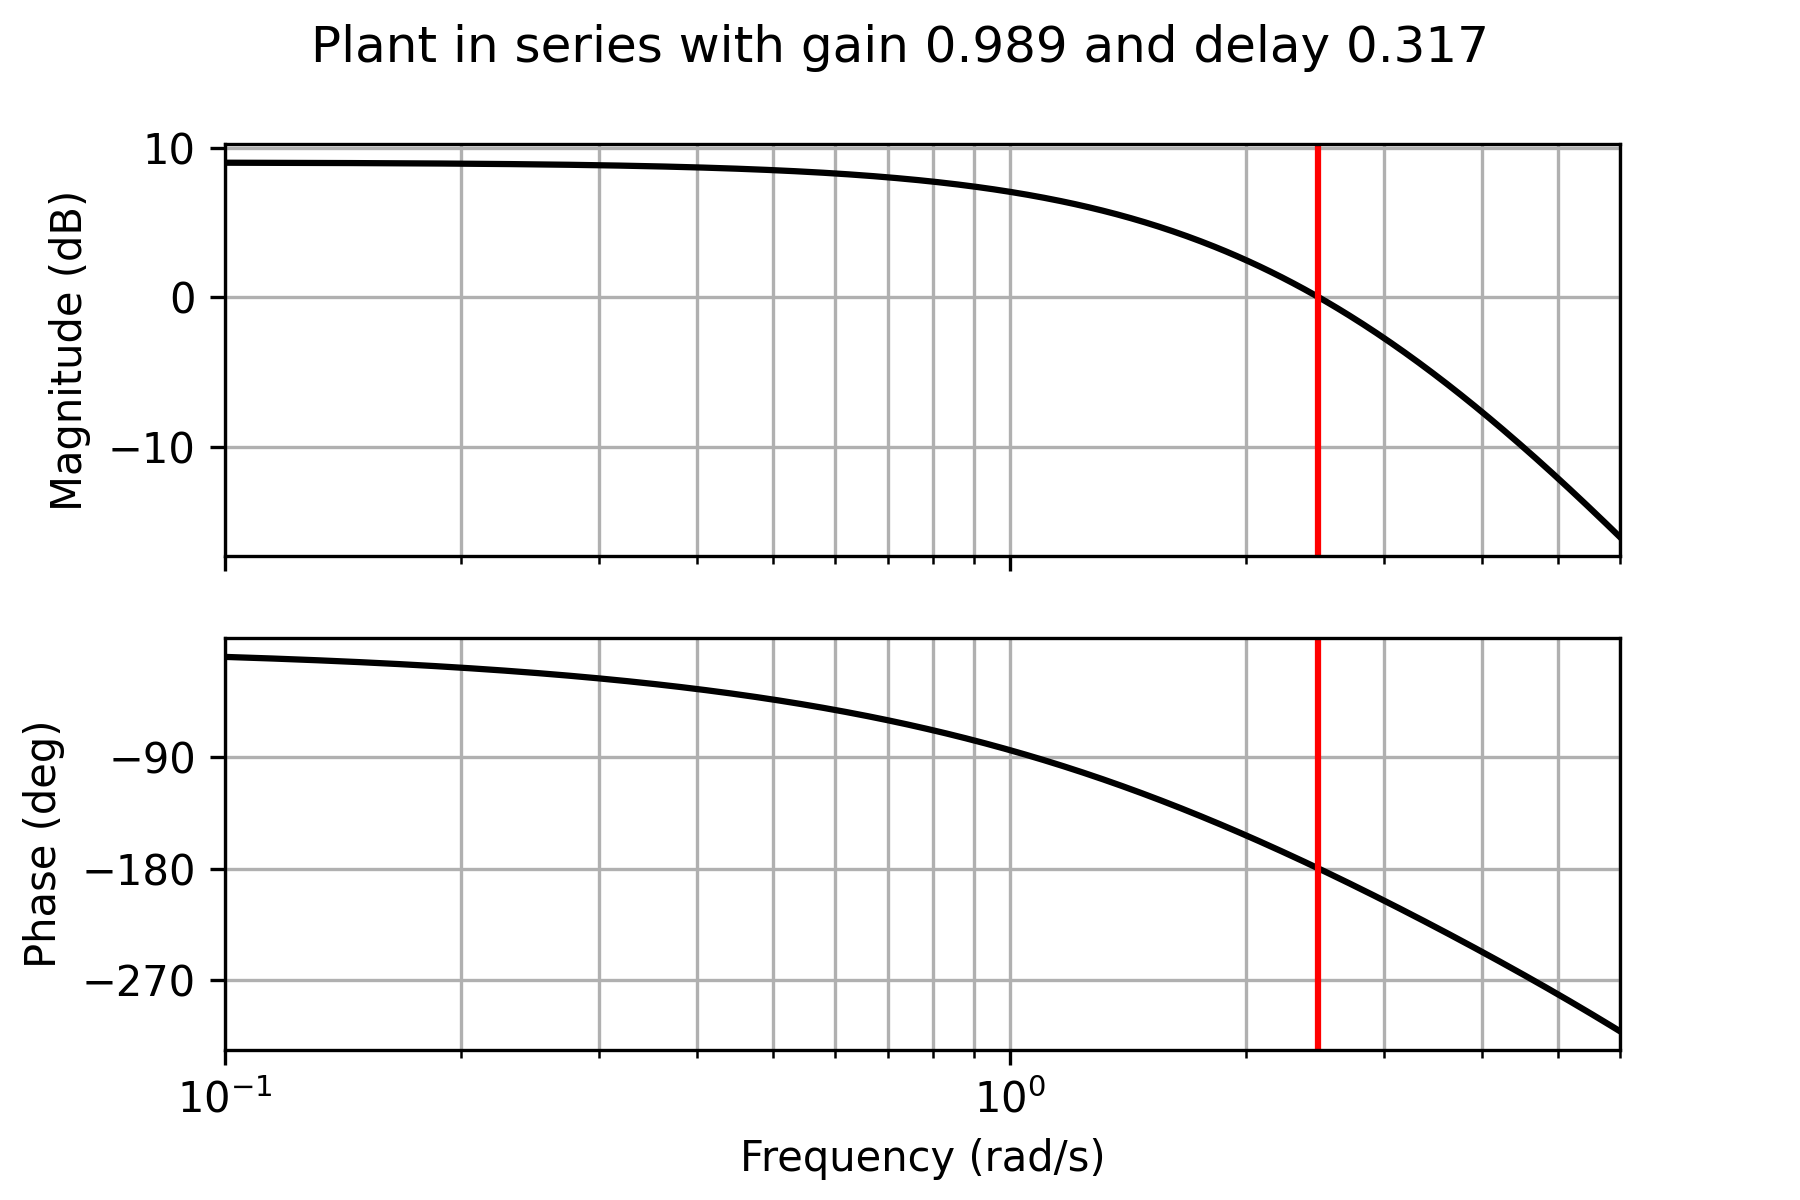
\includegraphics[width=0.8\textwidth]{figures/FIGURE_6.png}
    \caption{Figure 6}
    \label{fig:figure6}
\end{figure}

\begin{figure}
    \centering
    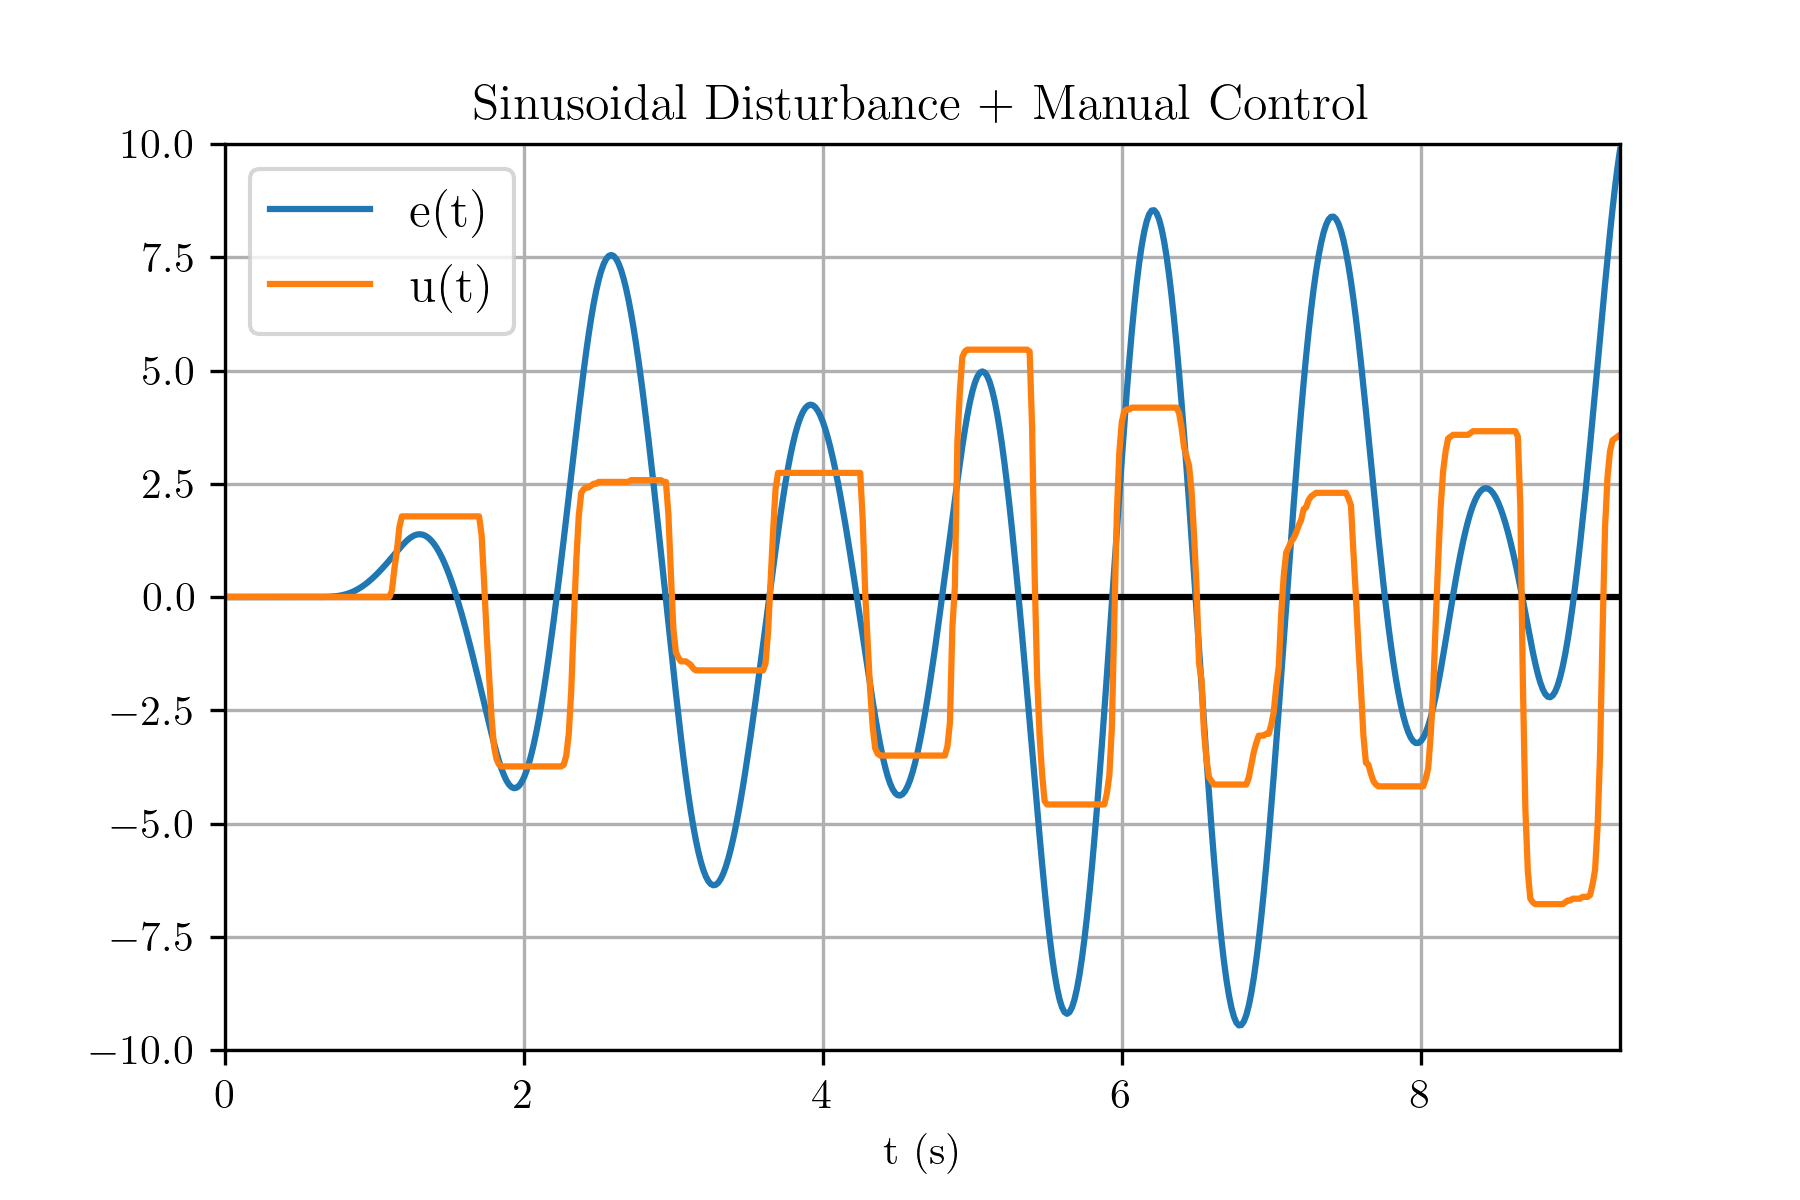
\includegraphics[width=0.8\textwidth]{figures/FIGURE_7.png}
    \caption{Figure 7}
    \label{fig:figure7}
\end{figure}

\newpage

\begin{figure}
    \centering
    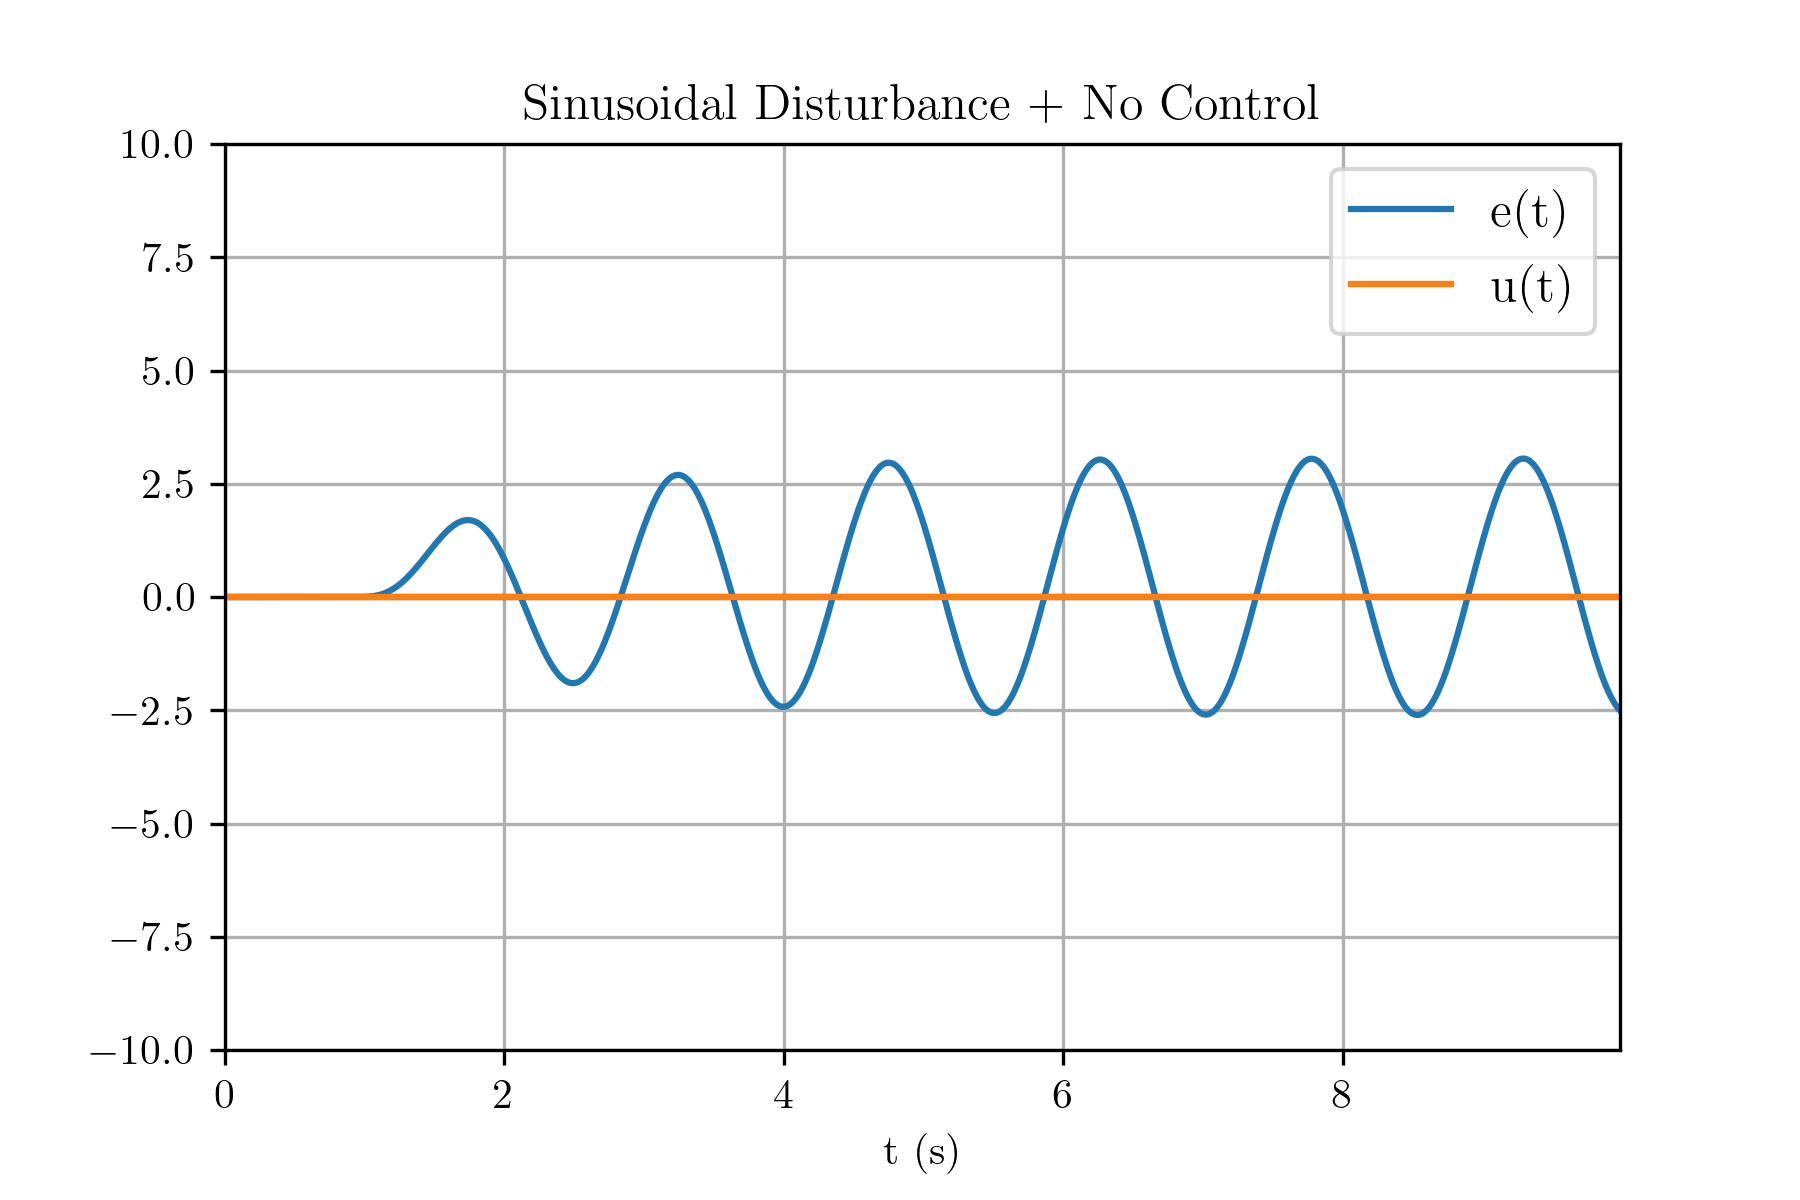
\includegraphics[width=0.8\textwidth]{figures/FIGURE_8.png}
    \caption{Figure 8}
    \label{fig:figure8}
\end{figure}

\begin{figure}
    \centering
    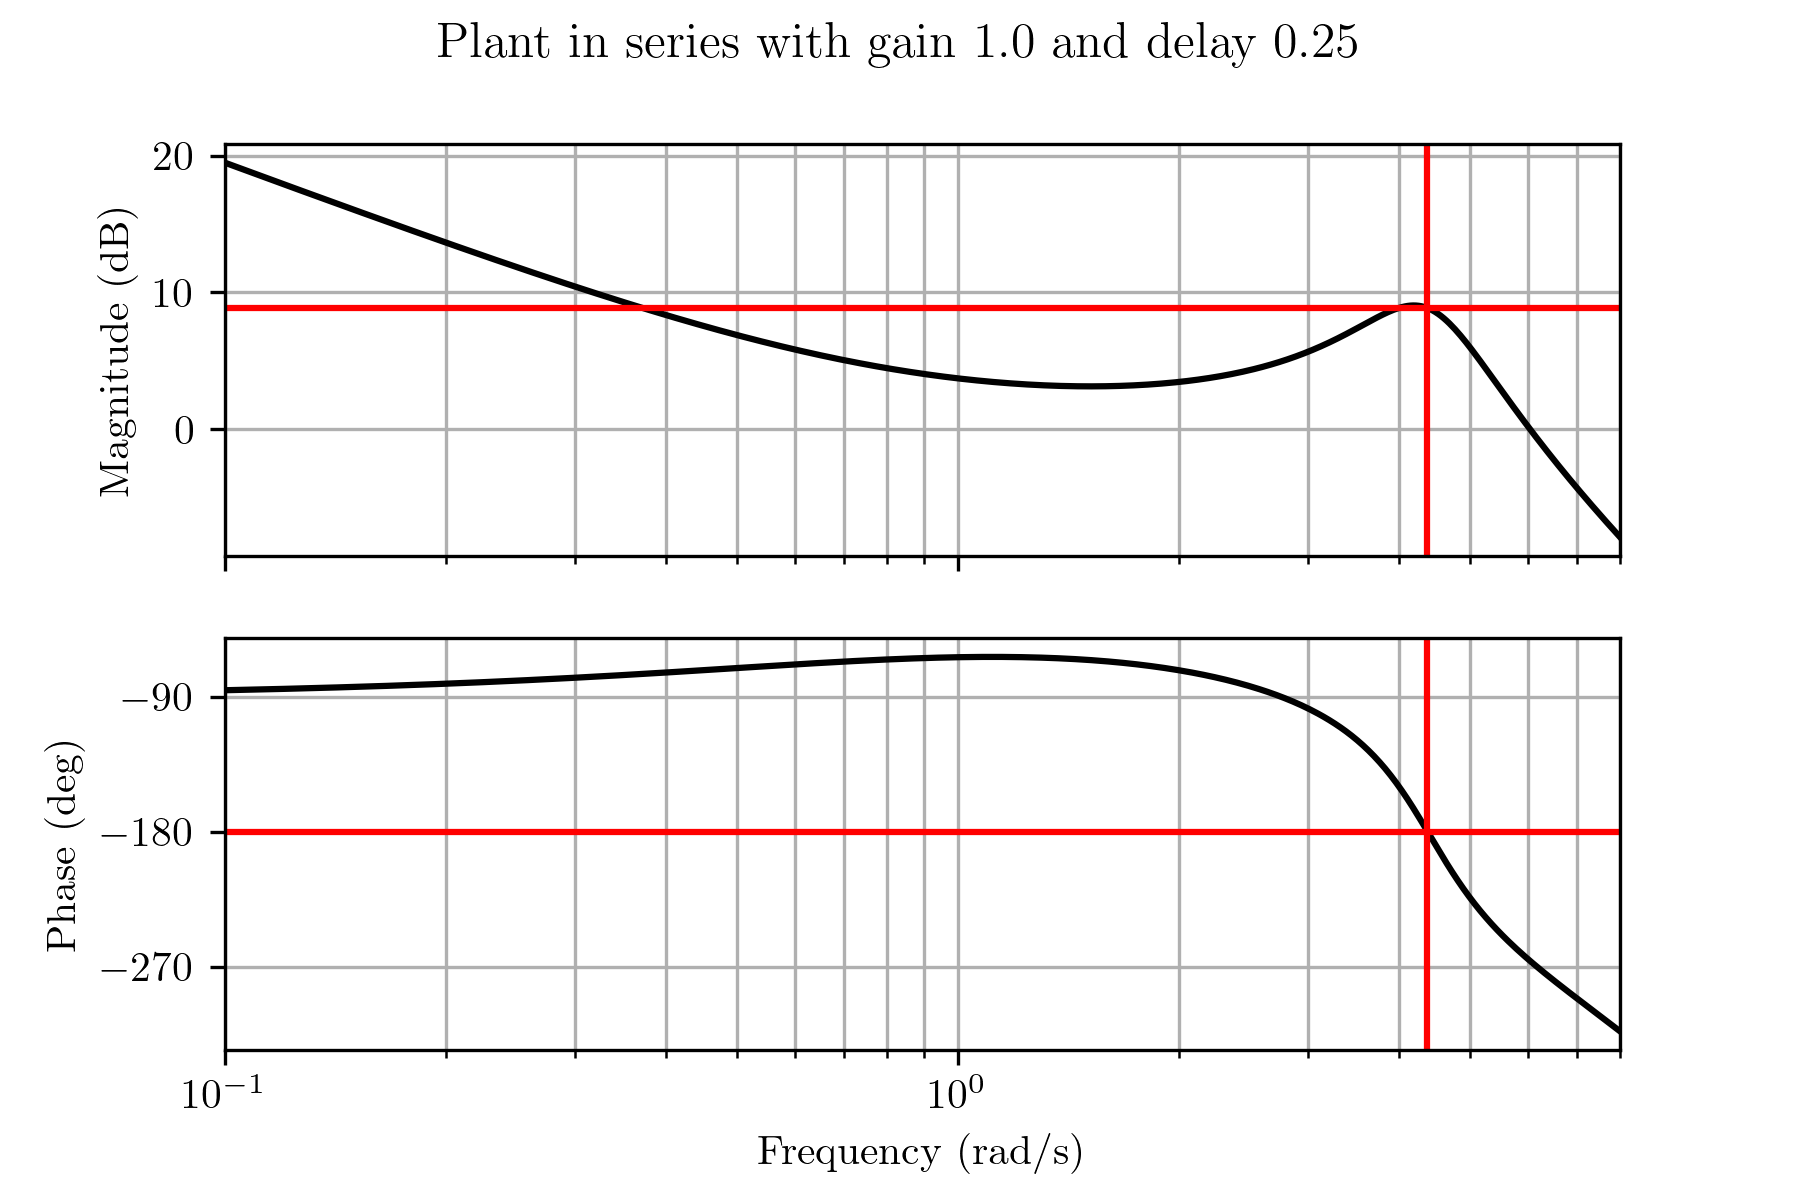
\includegraphics[width=0.8\textwidth]{figures/FIGURE_9.png}
    \caption{Figure 9}
    \label{fig:figure9}
\end{figure}

\newpage

\begin{figure}
    \centering
    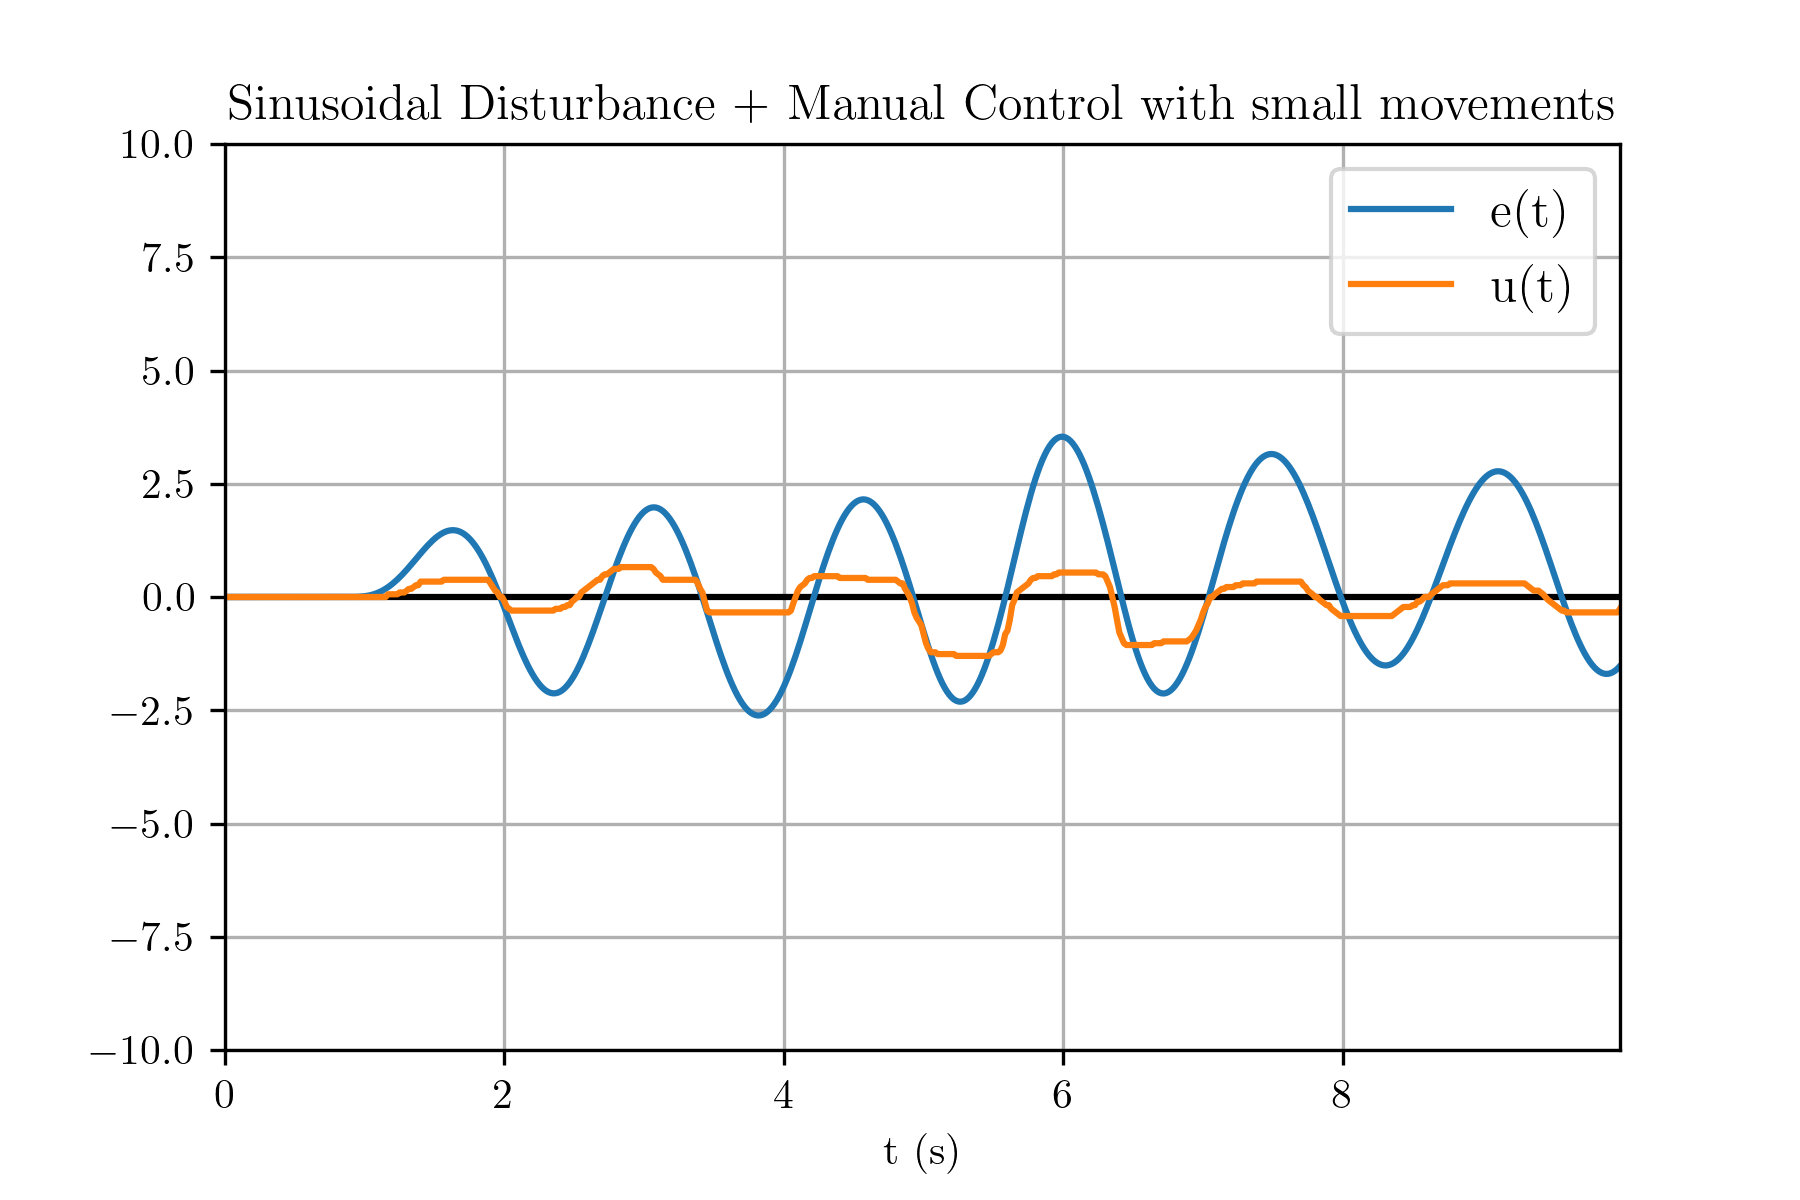
\includegraphics[width=0.8\textwidth]{figures/FIGURE_10.png}
    \caption{Figure 10}
    \label{fig:figure10}
\end{figure}

\begin{figure}
    \centering
    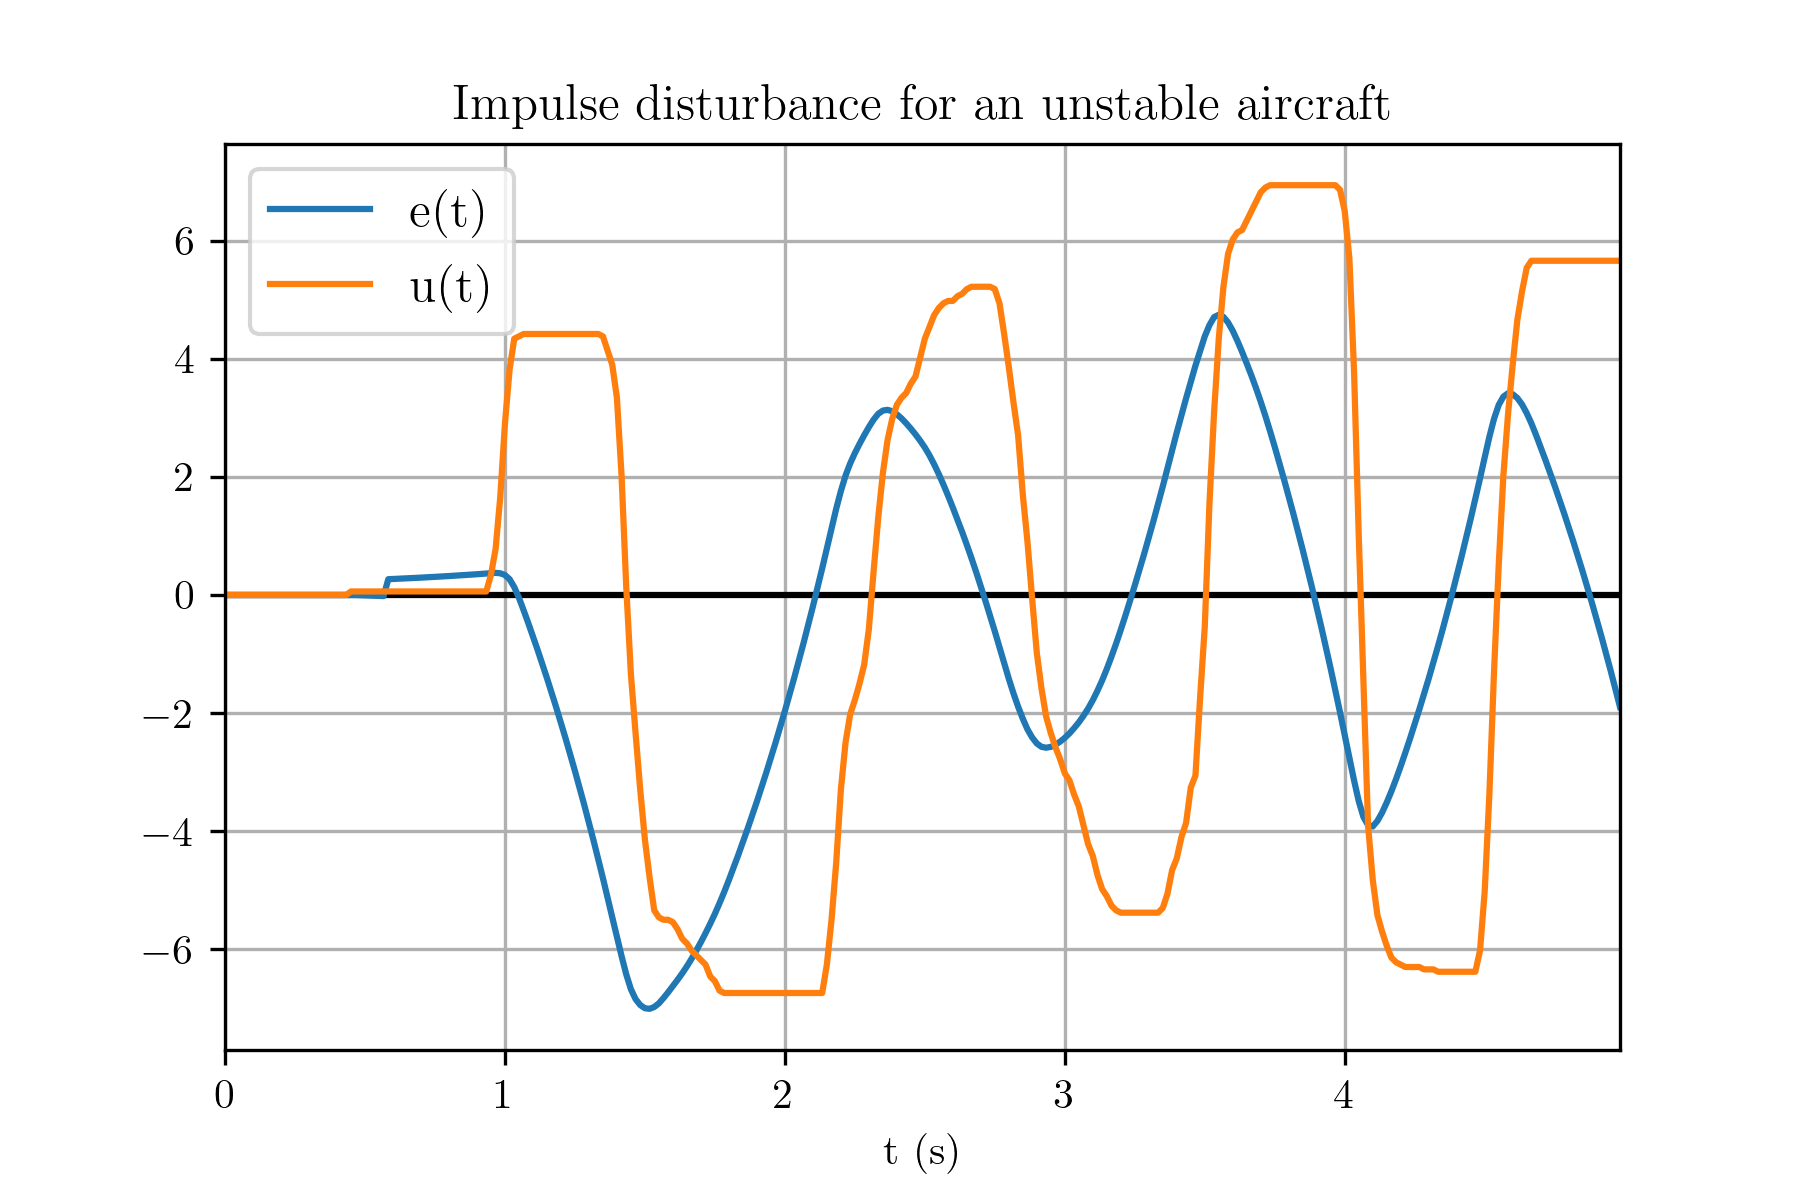
\includegraphics[width=0.8\textwidth]{figures/FIGURE_11.png}
    \caption{Figure 11}
    \label{fig:figure11}
\end{figure}

\newpage

\begin{figure}
    \centering
    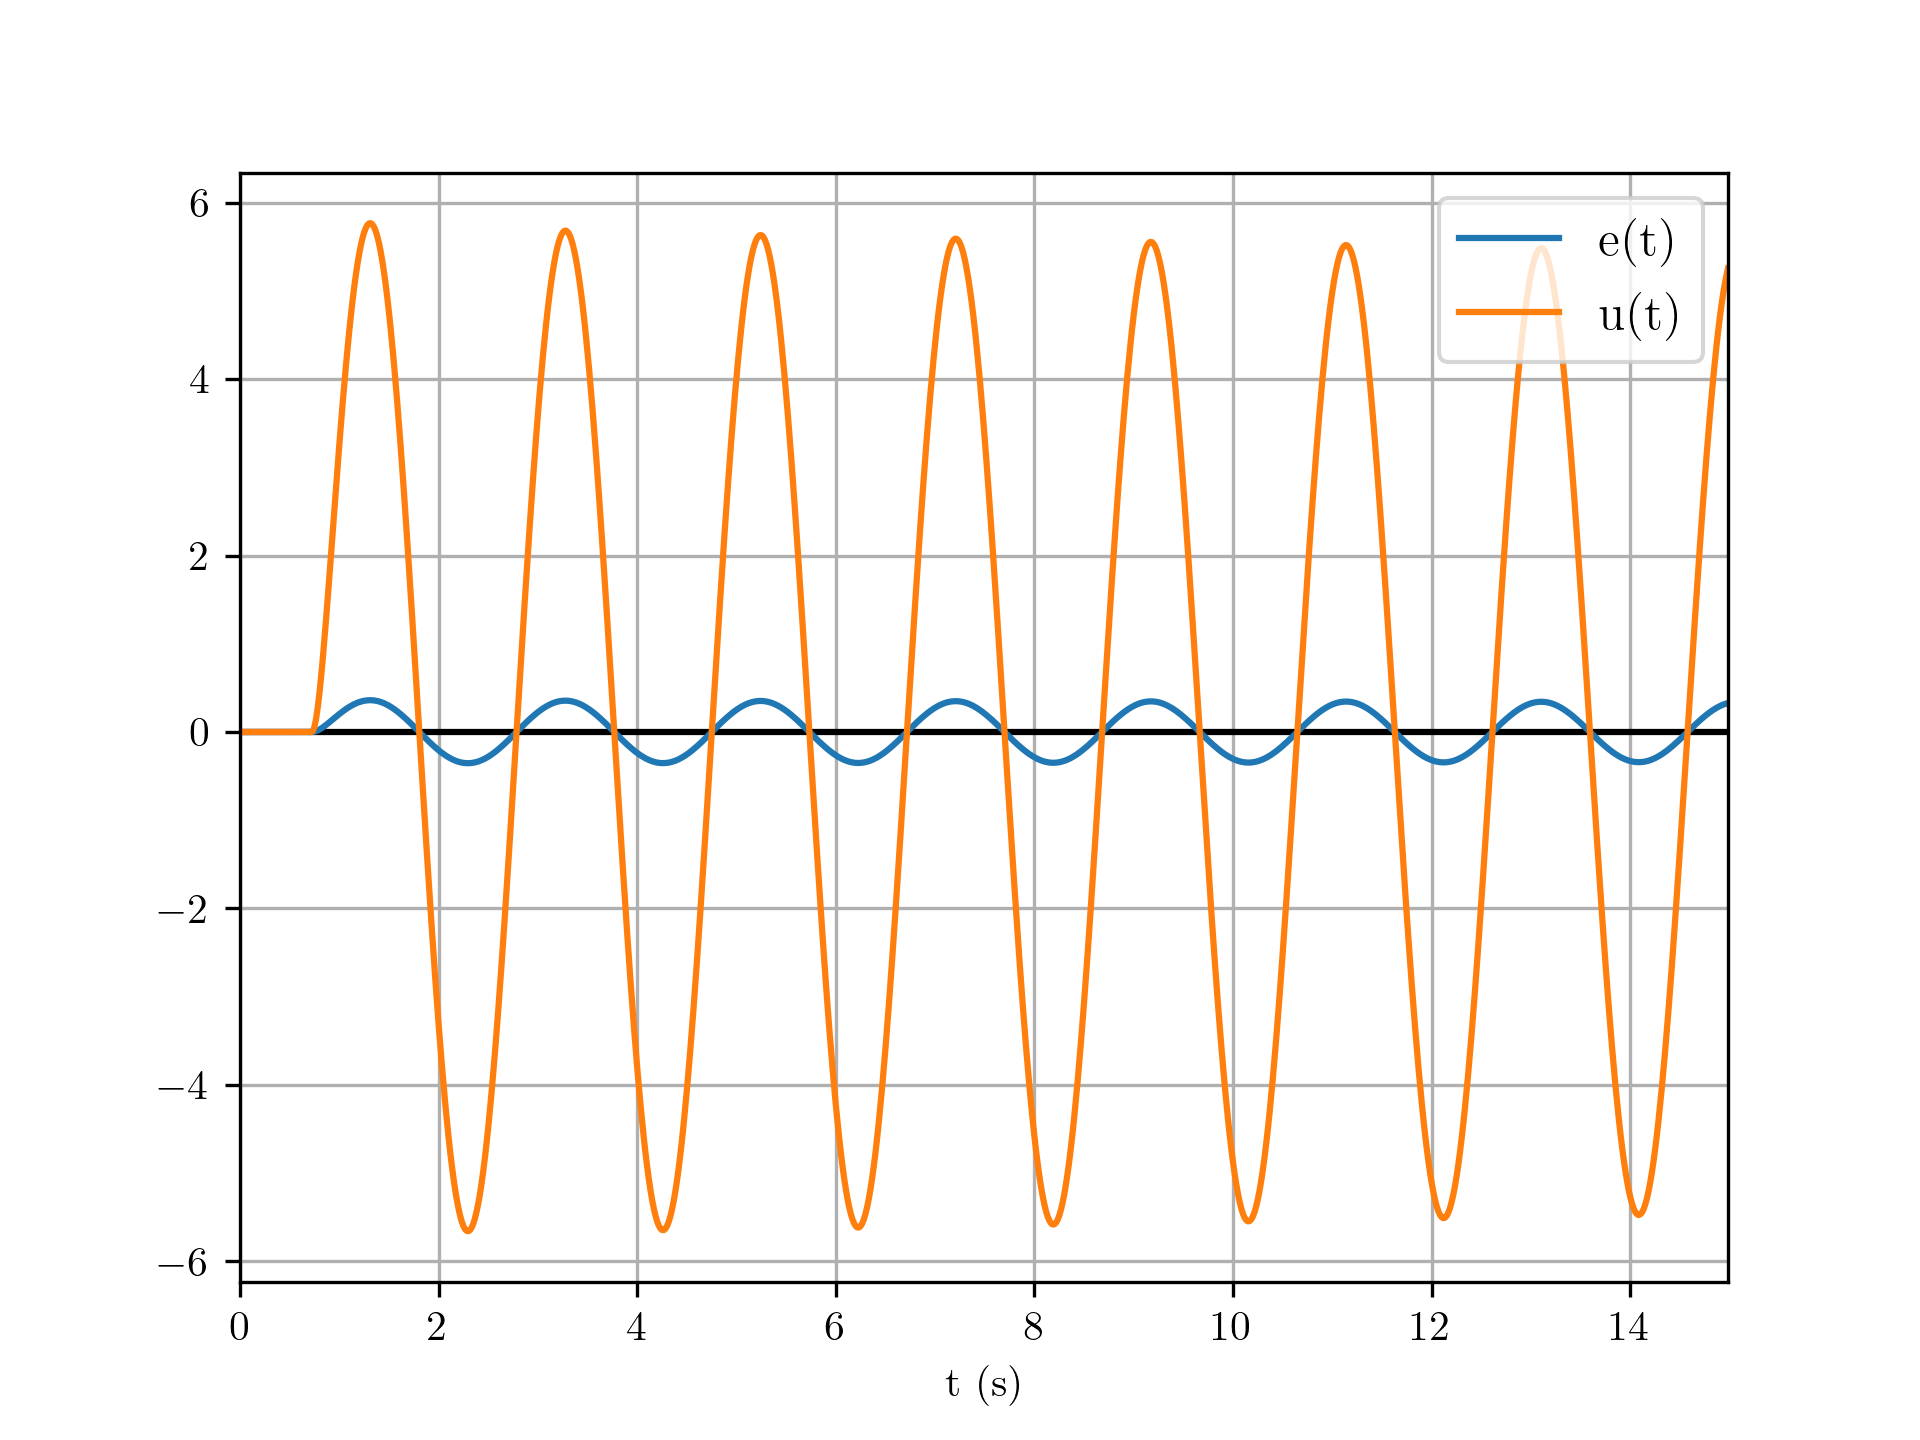
\includegraphics[width=0.8\textwidth]{figures/FIGURE_12.png}
    \caption{Figure 12}
    \label{fig:figure12}
\end{figure}

\begin{figure}
    \centering
    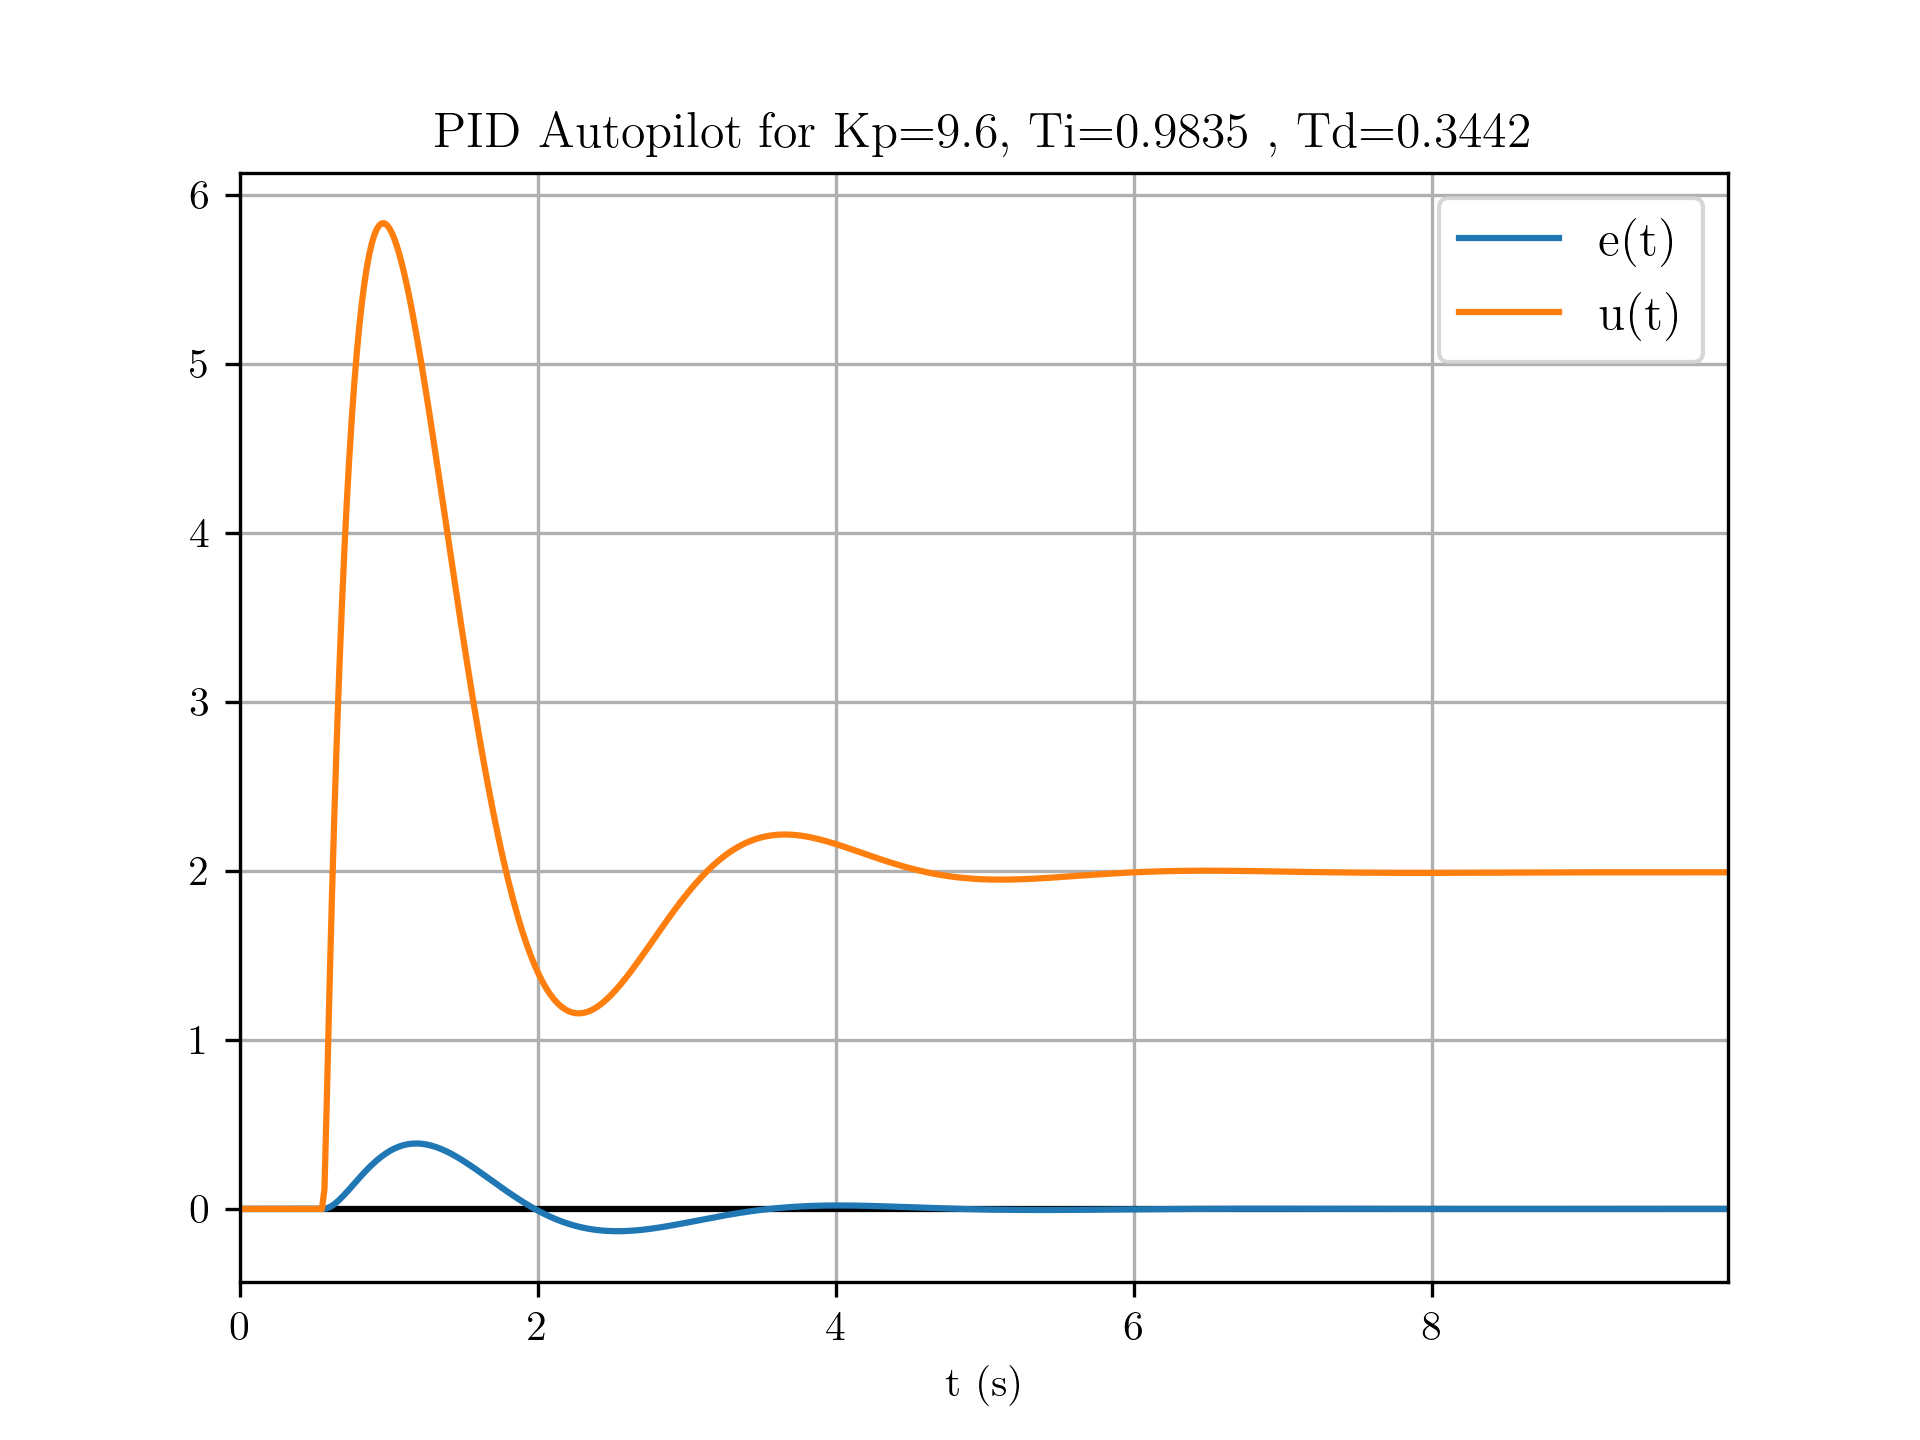
\includegraphics[width=0.8\textwidth]{figures/FIGURE_13.png}
    \caption{Figure 13}
    \label{fig:figure13}
\end{figure}

\newpage

\begin{figure}
    \centering
    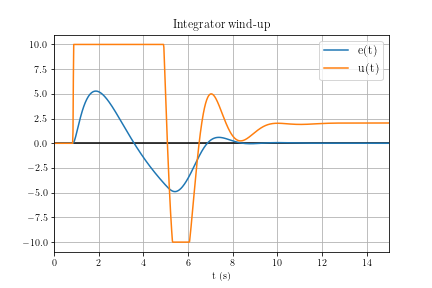
\includegraphics[width=0.8\textwidth]{figures/FIGURE_14.png}
    \caption{Figure 14}
    \label{fig:figure14}
\end{figure}

\begin{figure}
    \centering
    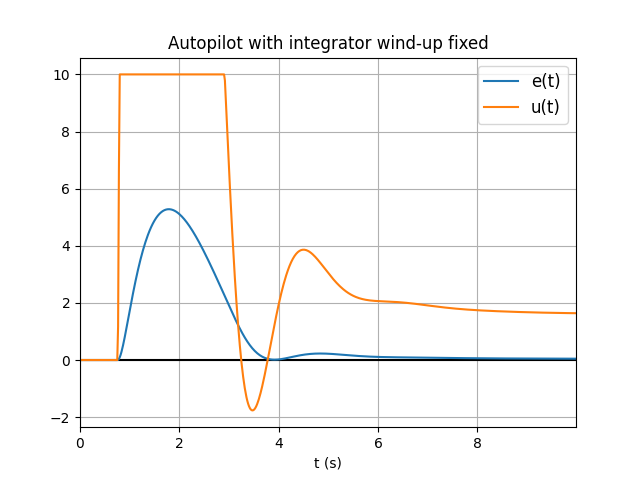
\includegraphics[width=0.8\textwidth]{figures/FIGURE_15.png}
    \caption{Figure 15}
    \label{fig:figure15}
\end{figure}

\newpage

\section{Discussion}

%interpret results and comment on anomalies

\subsection{Improvements}

\section{Conclusion}

From the experiments performed it can be observed that blah blah blah

\end{document}
